\documentclass{article}
\usepackage[T1]{fontenc}
\usepackage{lmodern}
\usepackage{graphicx}
\usepackage{amsmath,amssymb}
\usepackage[a4paper,margin=2cm]{geometry}
\usepackage[absolute,overlay]{textpos}
\setlength{\TPHorizModule}{1mm}
\setlength{\TPVertModule}{1mm}
\usepackage[indonesian]{babel}
\usepackage{hyperref}
\setlength{\emergencystretch}{2em}
% unit: Halaman 19

\begin{document}

% === Halaman 19 (llm) ===

\section*{Kebocoran data BPJS}

\vspace{50mm}

\begin{itemize}
    \item \textbf{KEBOCORAN DATA PRIBADI YANG TERUS BERULANG}
    \item DATA BPJS KESEHATAN BOCOR
    \begin{itemize}
        \item 279 juta data pengguna diperjualbelikan (Mei 2021)
        \item NIK nama, alamat, No phone, e-mail, foto
        \item Dijual di Raid Forums
        \item Harga jual 0.15 BTC (Rp 70-80 juta)
    \end{itemize}
    \item \textbf{Langkah pemerintah}
    \begin{itemize}
        \item Akses unduhan ditutup
        \item Bloker situs Raid Forums
        \item Investigasi
    \end{itemize}
    \item \textbf{KEBOCORAN DATA PERNAH TERJADI}
    \begin{itemize}
        \item Kasus 2020
        \begin{itemize}
            \item 91 juta data pengguna \& 7 juta data merchant (Tokopedia)
            \item 2,3 juta data pemilih Pemilu 2014 (KPU)
            \item 250 ribu data pasien Covid-19
        \end{itemize}
    \end{itemize}
    \item \textbf{Pentingnya regulasi}
    \begin{itemize}
        \item Masyarakat berhak:
        \begin{itemize}
            \item Tahu tujuan penggunaan data
            \item Hapus data ke pengelola
        \end{itemize}
        \item Pengelola wajib mitigasi kebocoran
        \item Sanksi/denda jika bocor
        \end{itemize}
    \end{itemize}
\end{itemize}

% deskripsi: Screenshot forum gelap yang menunjukkan postingan penjualan data warga negara Indonesia (NIK, KTP, Phone, dll) oleh pengguna bernama 'kotz'.
% bbox normalisasi: [0.0700, 0.1800, 0.5770, 0.7210]
\begin{textblock*}{106.47mm}(14.70mm,53.46mm)
\noindent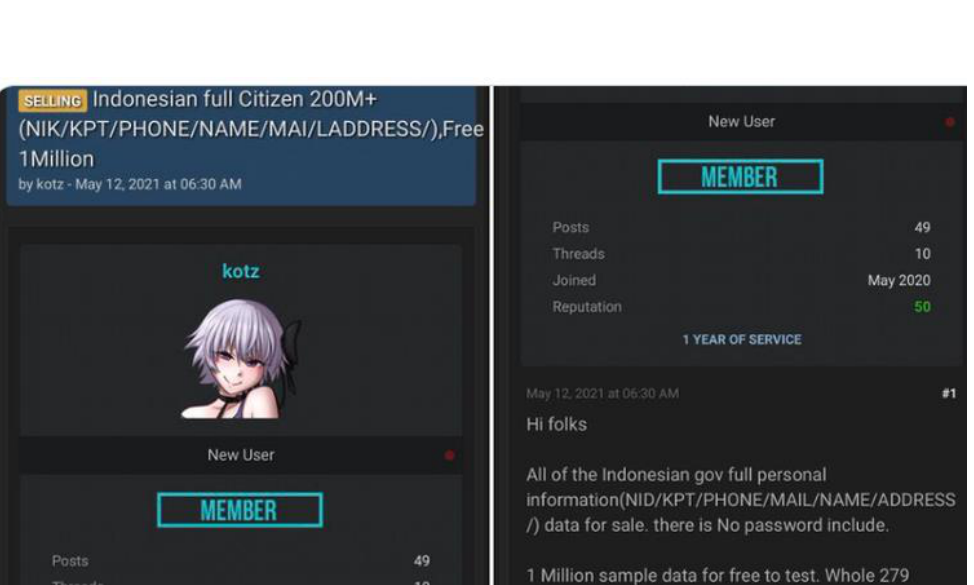
\includegraphics[width=106.47mm,height=160.68mm]{../../images/llm/page_019_img_01.png}%
\end{textblock*}

% deskripsi: Ilustrasi visual berupa tumpukan kertas dokumen yang diberi cap 'TOP SECRET' sebagai representasi kebocoran data.
% bbox normalisasi: [0.6140, 0.3280, 0.7600, 0.6560]
\begin{textblock*}{30.66mm}(128.94mm,97.42mm)
\noindent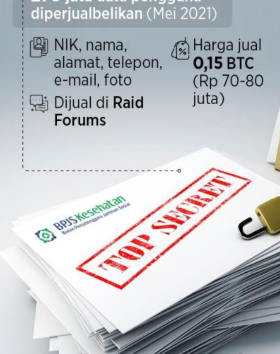
\includegraphics[width=30.66mm,height=97.42mm]{../../images/llm/page_019_img_02.png}%
\end{textblock*}

\end{document}
